\title{CSC 458 Assignment 1}
\author{Nick Graham}
\date{\today}

\documentclass[12pt]{article}

\usepackage{graphicx}

\begin{document}
\maketitle

\section*{Introduction}
Assignment One had us look at the default C++
implementatiom of threads that were introduced in C++
11. It had us use the threads in 5 different cases that
utilized different syncronization methods. The methods
that were tested include nothing at all, a mutex with
implecit lock and unlock calls, the C++ lock\_gaurd, an
atomic integer with fetch and add, and then a method
which gave each thread its own counter, and then the
main thread combined the results.

\section*{No Syncronization}
When not using syncronization there were numerous tests
that returned the incorrect results, although it
complete in a reasonably short amount of time.

The results were incorrect because threads were accessing the memory location at the same time, and not able to exectute atomically.

For 16 Threads, 1 Million Increments

The average time spent: 0.7327239999999999 sec

The average result: 13253086

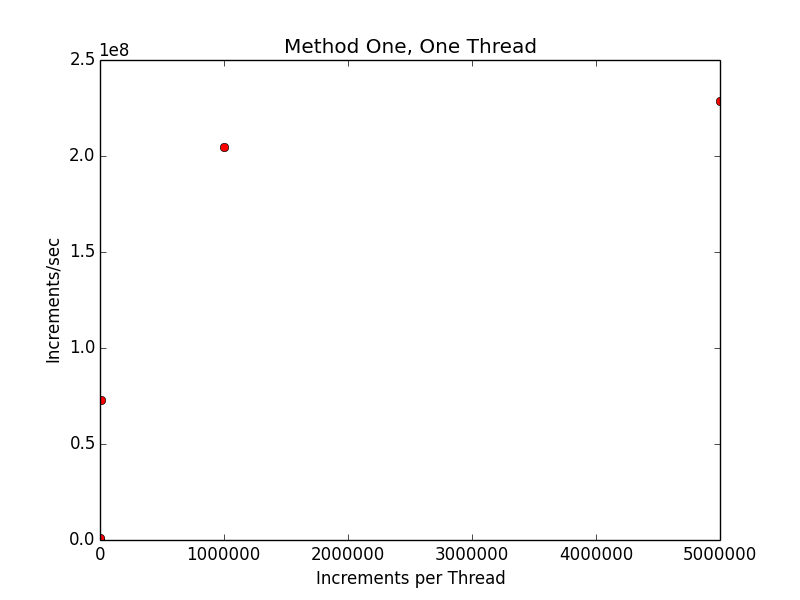
\includegraphics[scale=.5]{Graphs/MethodOne_1Thread.png}

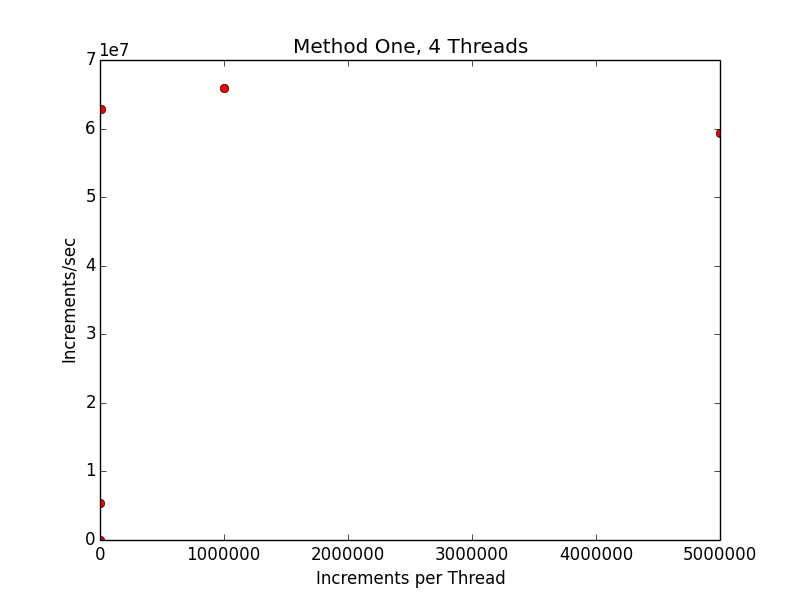
\includegraphics[scale=.5]{Graphs/MethodOne_4Thread.png}

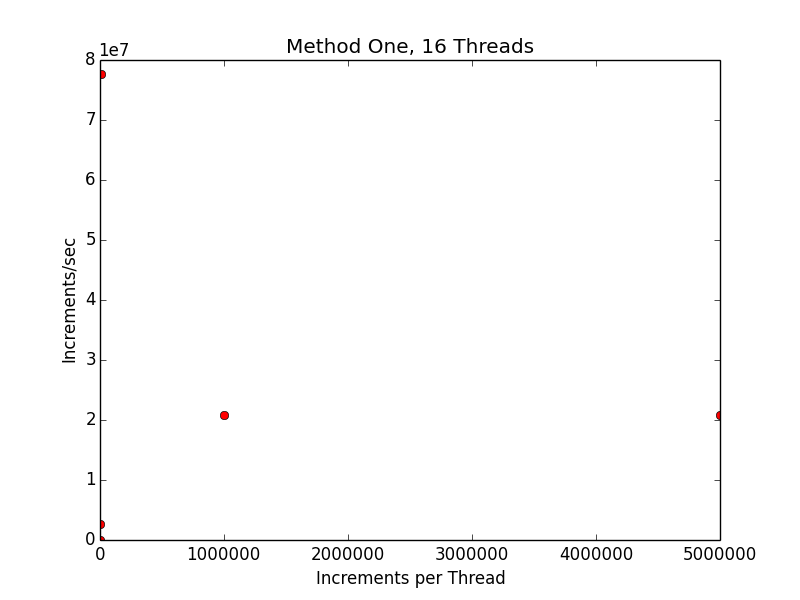
\includegraphics[scale=.5]{Graphs/MethodOne_16Thread.png}

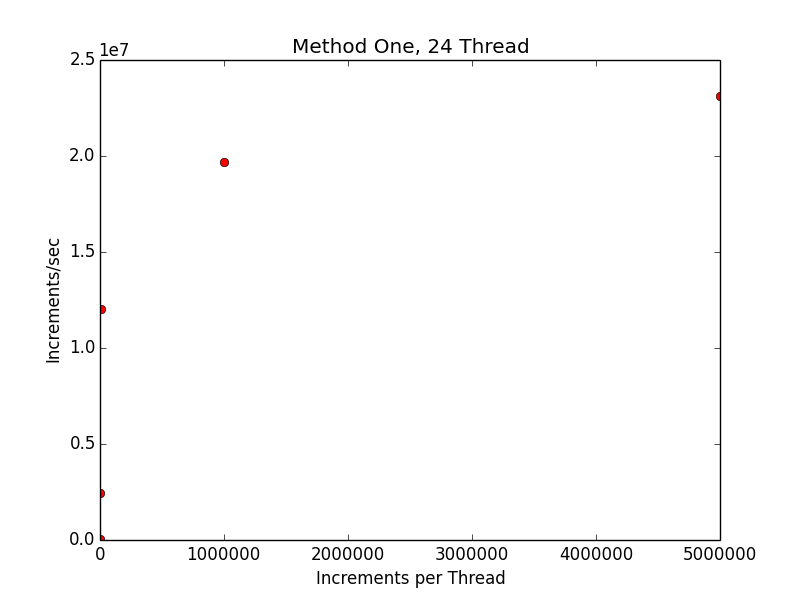
\includegraphics[scale=.5]{Graphs/MethodOne_24Thread.png}

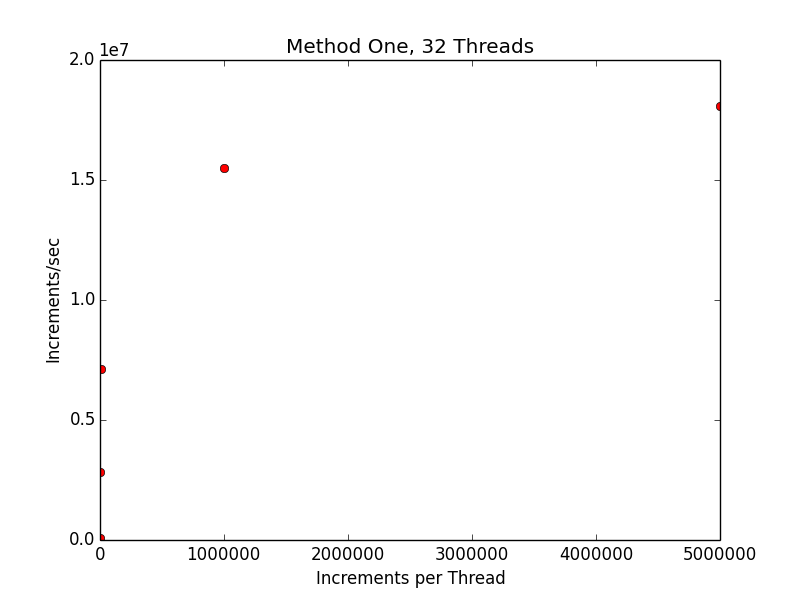
\includegraphics[scale=.5]{Graphs/MethodOne_32Thread.png}

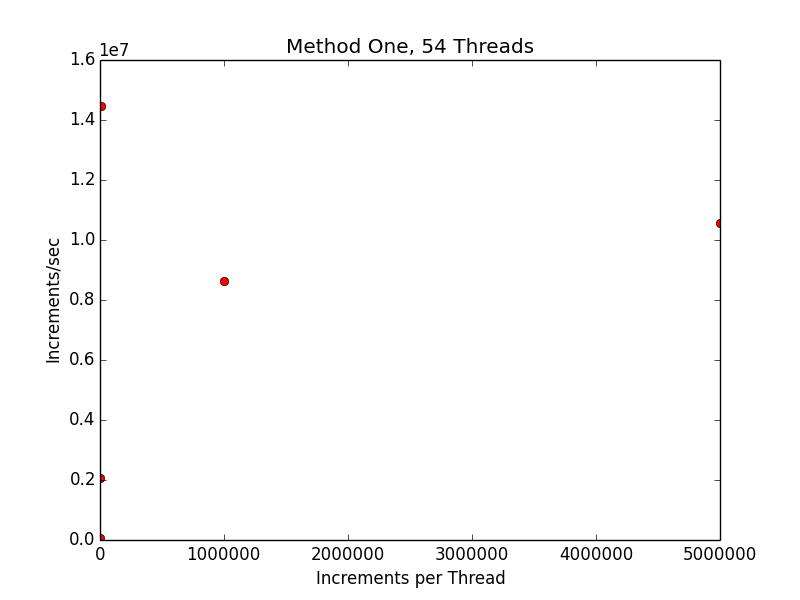
\includegraphics[scale=.5]{Graphs/MethodOne_54Thread.png}


\section*{Explicite Lock and Unlock}
Using a mutex with explicite lock and unlock calls
fixed the correctness issues that were seen when not
using Syncronization, but they increased the runtime.
This increase in runtime is most likely due to the added atomic
calls that need to be made to gain acess to the mutex.

For 16 Threads, 1 Million Increments

The average time spent: 35.22414 sec

The average result: 160000000

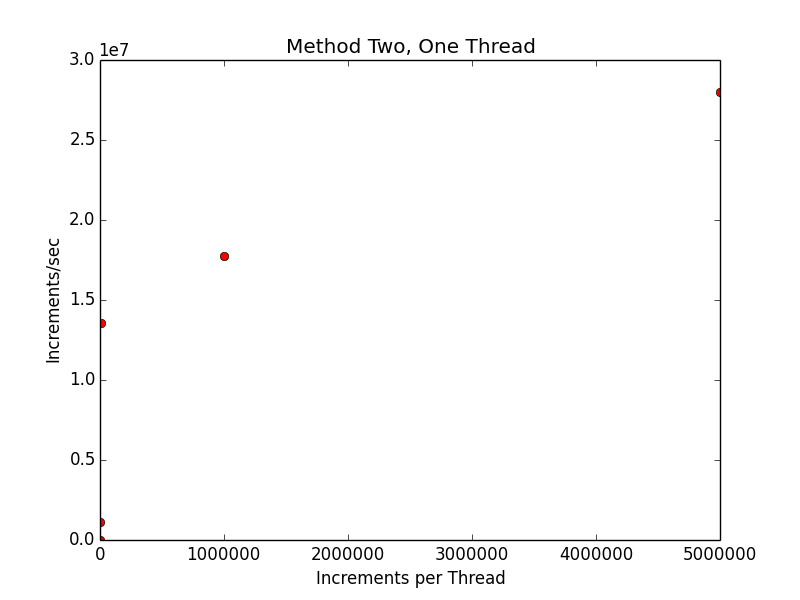
\includegraphics[scale=.5]{Graphs/MethodTwo_1Thread.png}

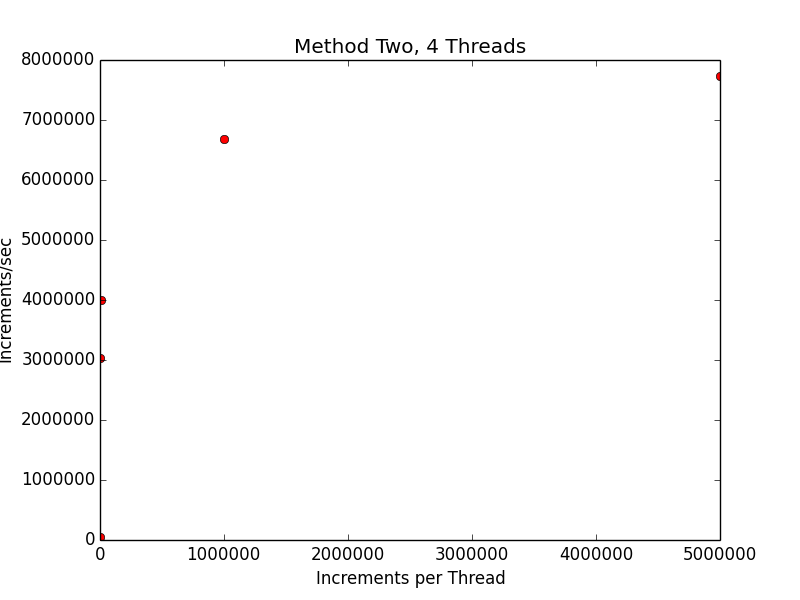
\includegraphics[scale=.5]{Graphs/MethodTwo_4Thread.png}

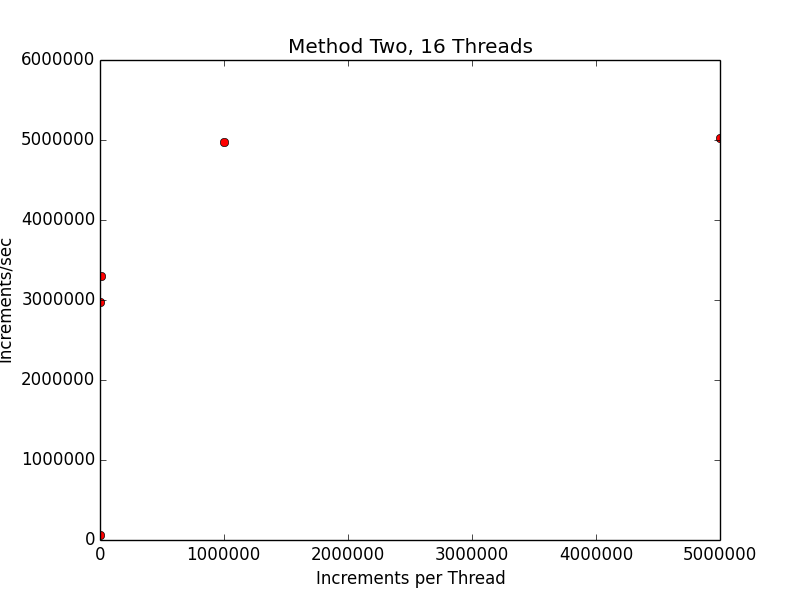
\includegraphics[scale=.5]{Graphs/MethodTwo_16Thread.png}

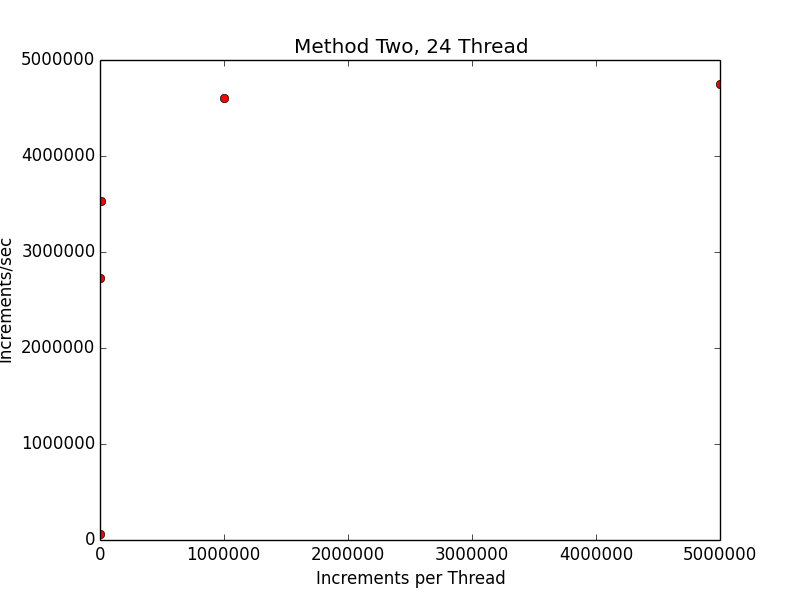
\includegraphics[scale=.5]{Graphs/MethodTwo_24Thread.png}

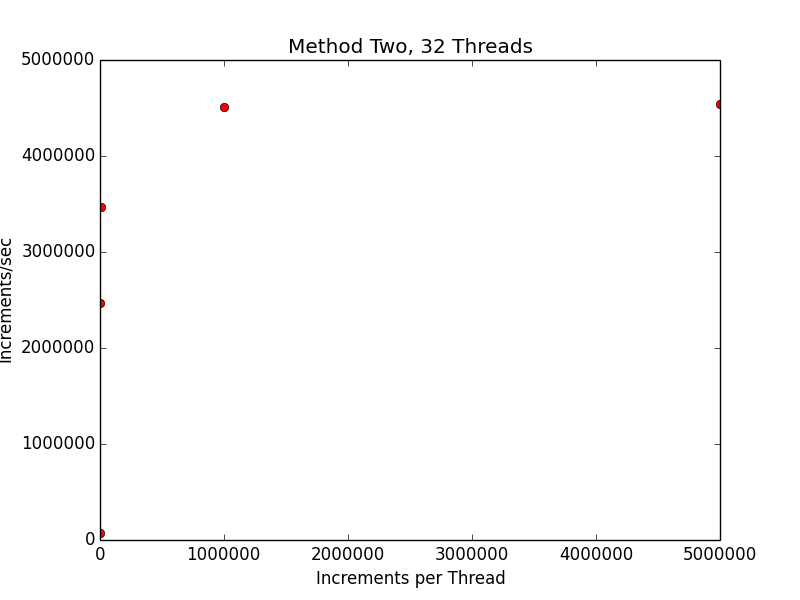
\includegraphics[scale=.5]{Graphs/MethodTwo_32Thread.png}

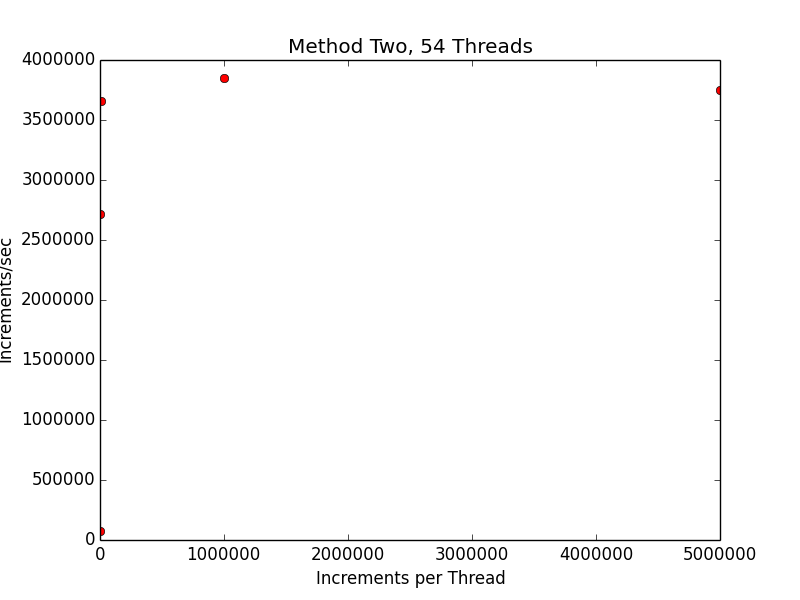
\includegraphics[scale=.5]{Graphs/MethodTwo_54Thread.png}


\section*{Lock Gaurd}
Using a mutex with a call to lock guard tended to be
worse then the explicite calls to lock and unlock,
although not by much. This is most likely due to the fact that
even though the number of atomic calls written to the mutex
was cut in half from the previous method, the call to release
the lock was still there.

For 16 Threads, 1 Million Increments

The average time spent: 38.27466 sec

The average result: 160000000


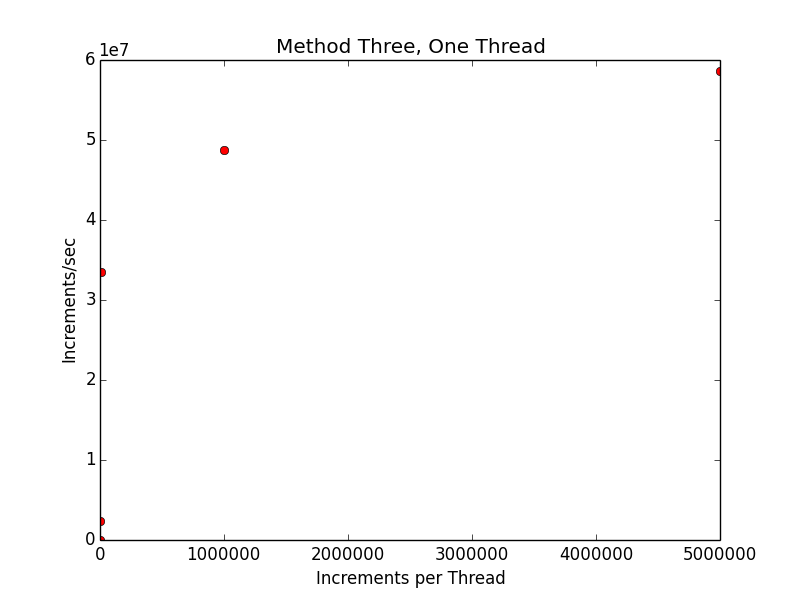
\includegraphics[scale=.5]{Graphs/MethodThree_1Thread.png}

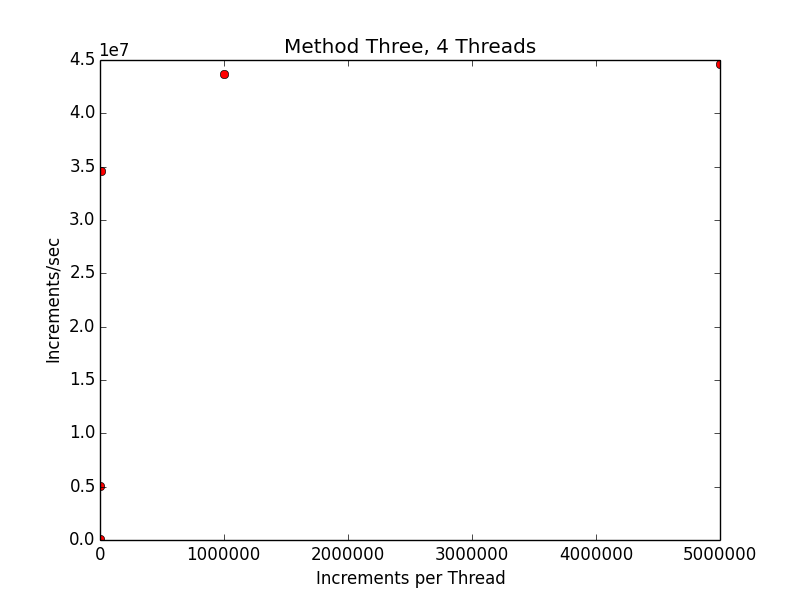
\includegraphics[scale=.5]{Graphs/MethodThree_4Thread.png}

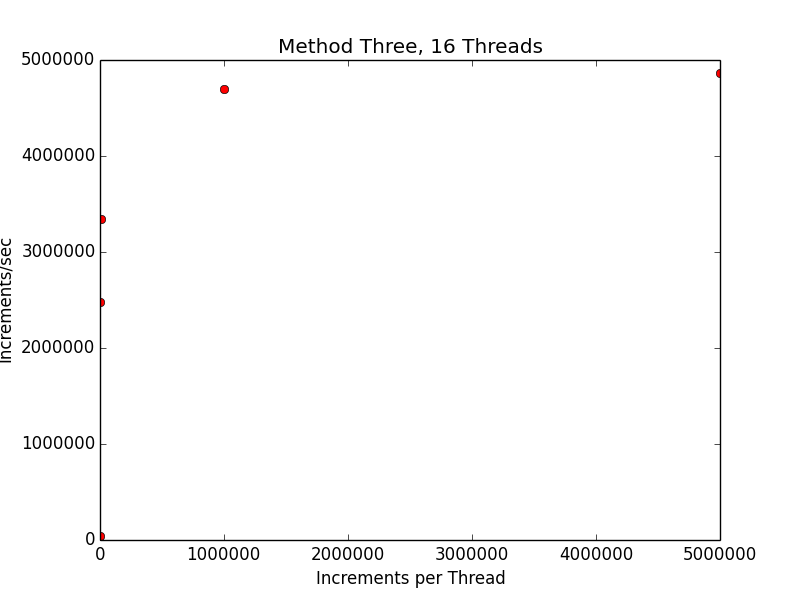
\includegraphics[scale=.5]{Graphs/MethodThree_16Thread.png}

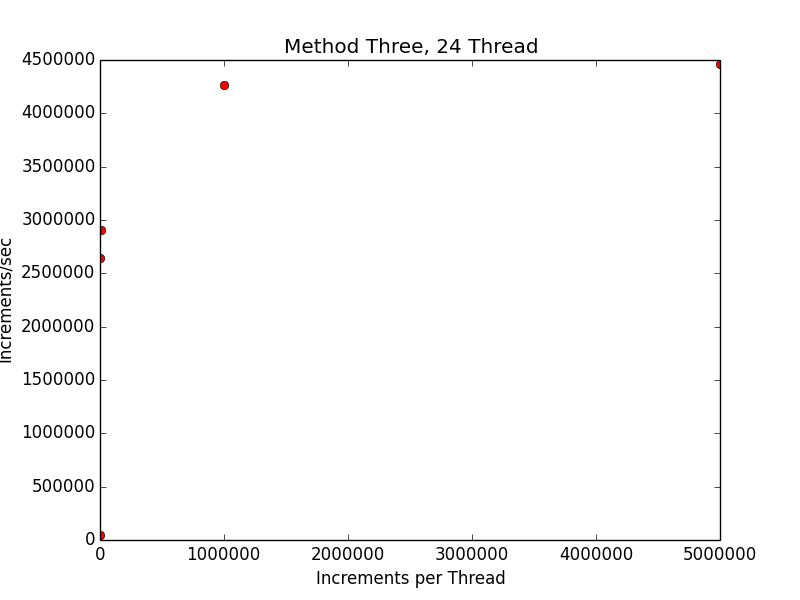
\includegraphics[scale=.5]{Graphs/MethodThree_24Thread.png}

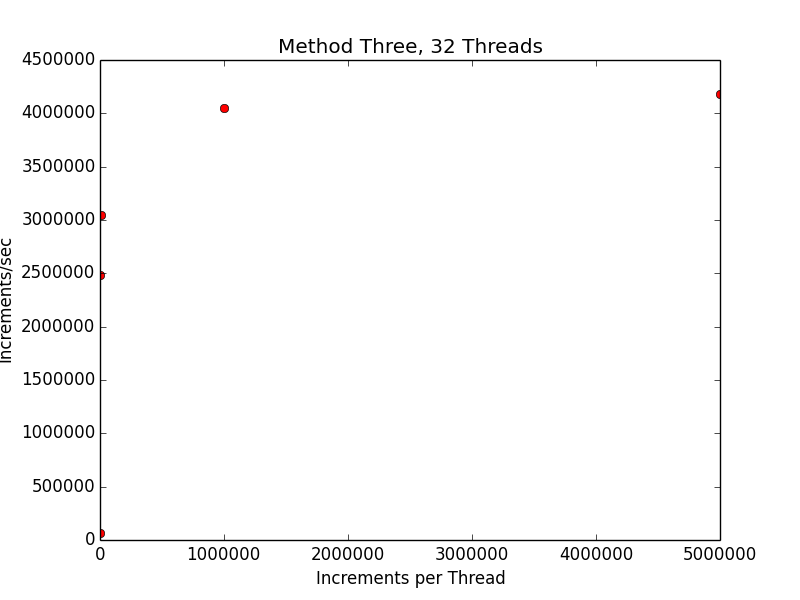
\includegraphics[scale=.5]{Graphs/MethodThree_32Thread.png}

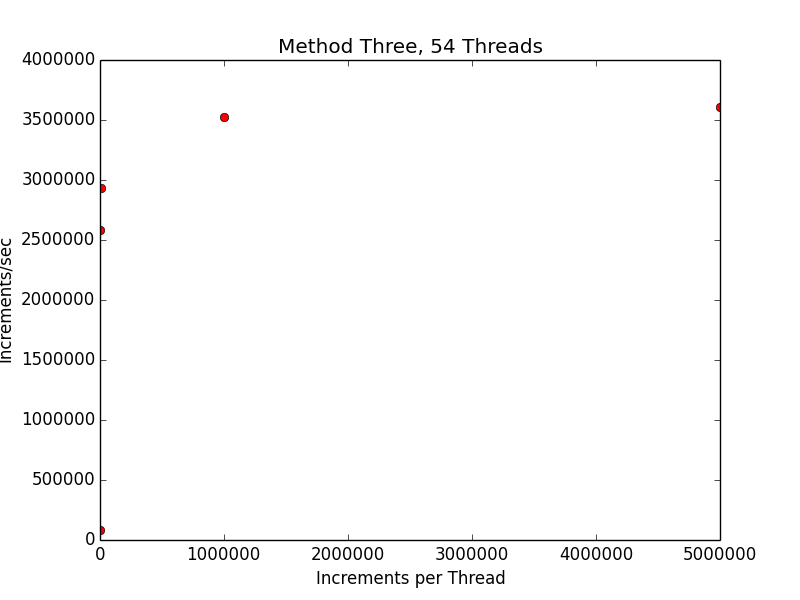
\includegraphics[scale=.5]{Graphs/MethodThree_54Thread.png}


\section*{Atomic Integer}
Using an atomic integer also executed correctly, and
was much faster then both mutex implementations. I believe this
is because instead of needing to make multiple atomic calls to
a mutex, you only have to make an atomic call when you are updating
the counter.

For 16 Threads, 1 Million Increments

The average time spent: 3.3682299999999996 sec

The average result: 160000000

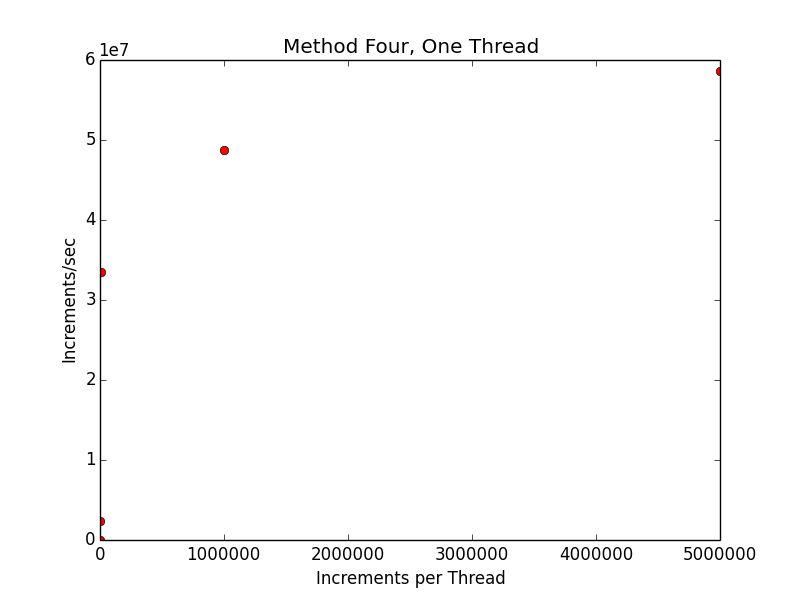
\includegraphics[scale=.5]{Graphs/MethodFour_1Thread.png}

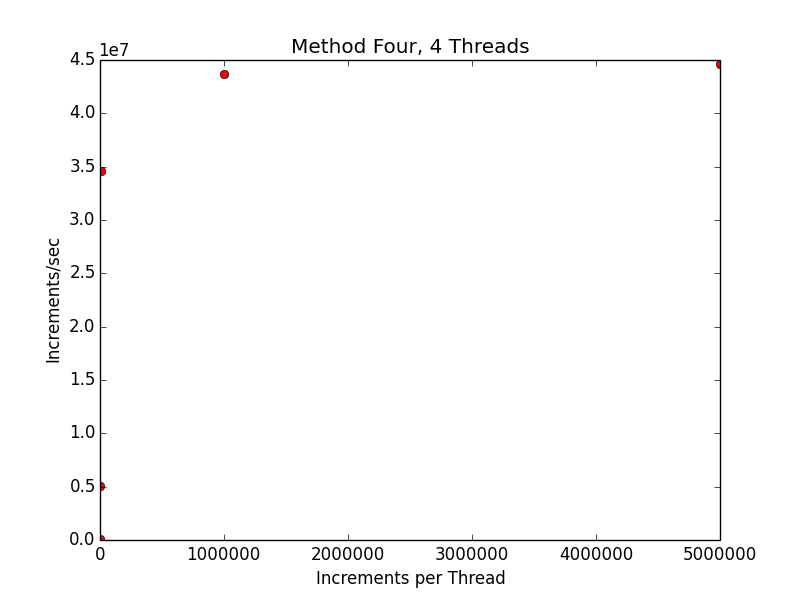
\includegraphics[scale=.5]{Graphs/MethodFour_4Thread.png}

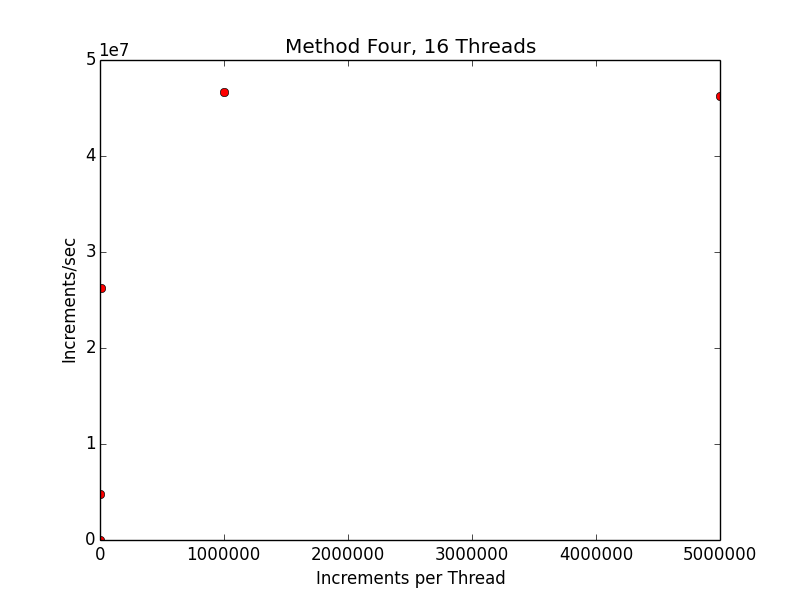
\includegraphics[scale=.5]{Graphs/MethodFour_16Thread.png}

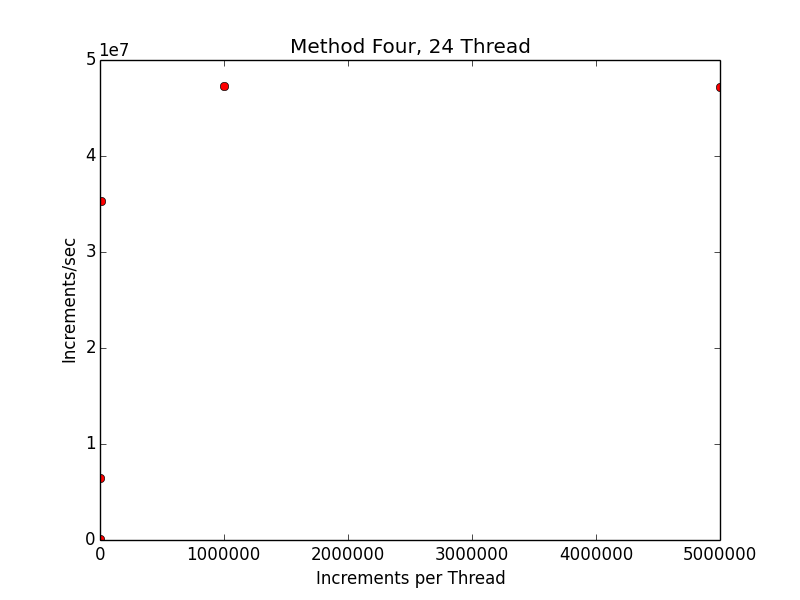
\includegraphics[scale=.5]{Graphs/MethodFour_24Thread.png}

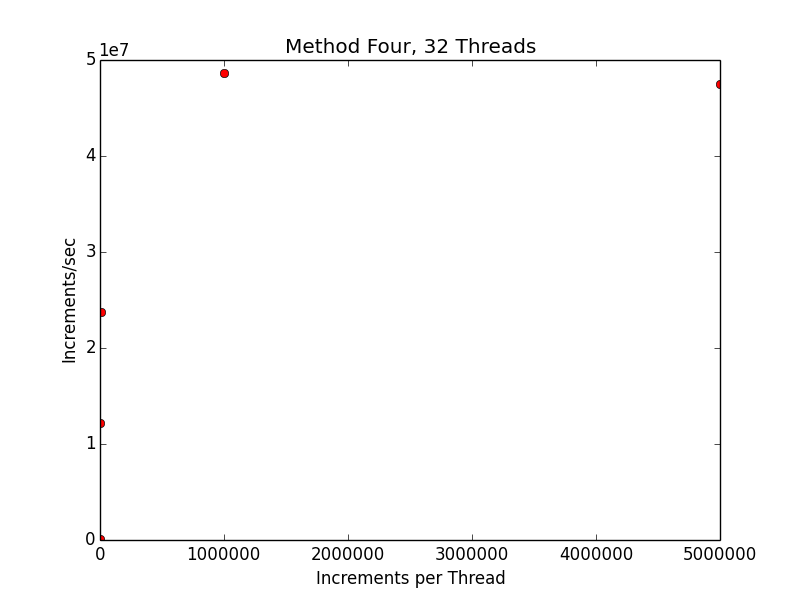
\includegraphics[scale=.5]{Graphs/MethodFour_32Thread.png}

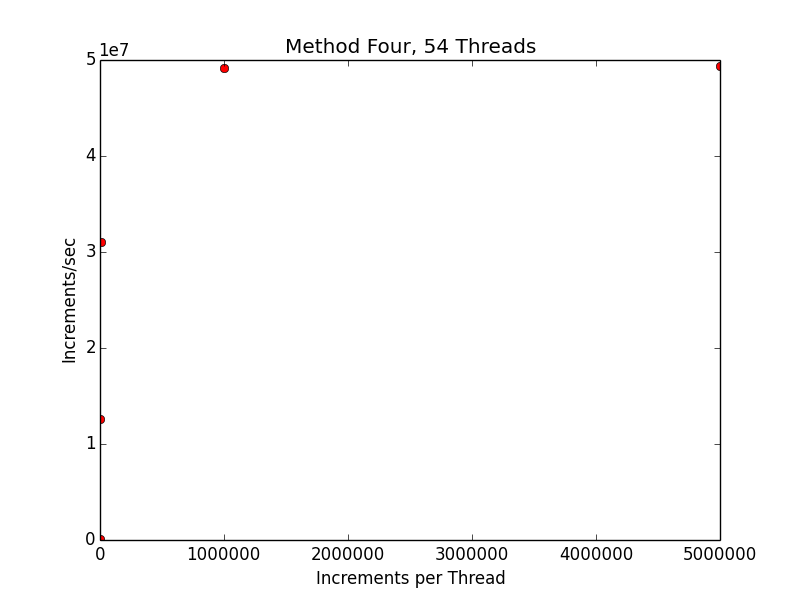
\includegraphics[scale=.5]{Graphs/MethodFour_54Thread.png}


\section*{Seperate Threads}
Creating seperate threads executed correctly, and was
much faster then the mutex implementations. I believe this is
because it requires no atomic operations, since each thread operates
on a local variable. This has comparable runtime to the first method,
with a small amount of overhead in the main thread.

For 16 Threads, 1 Million Increments

The average time spent: 0.49986600000000003 sec

The average result: 160000000

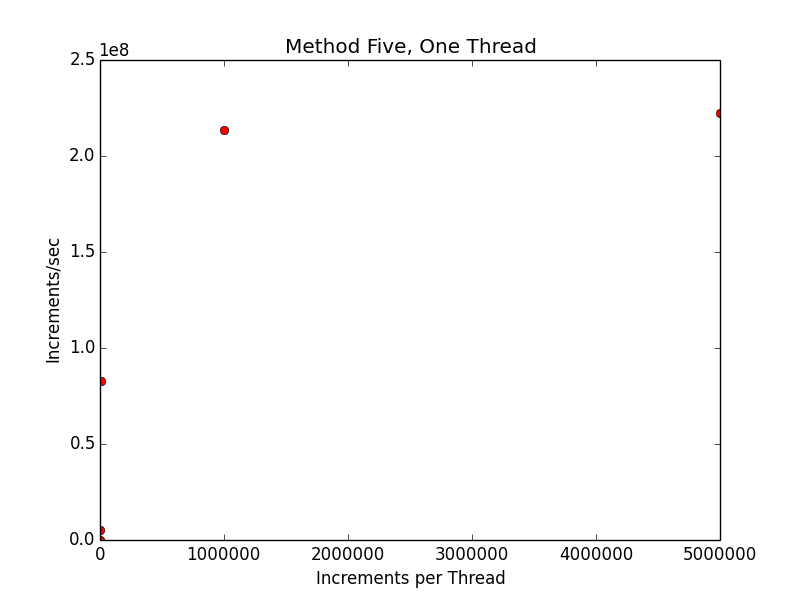
\includegraphics[scale=.5]{Graphs/MethodFive_1Thread.png}

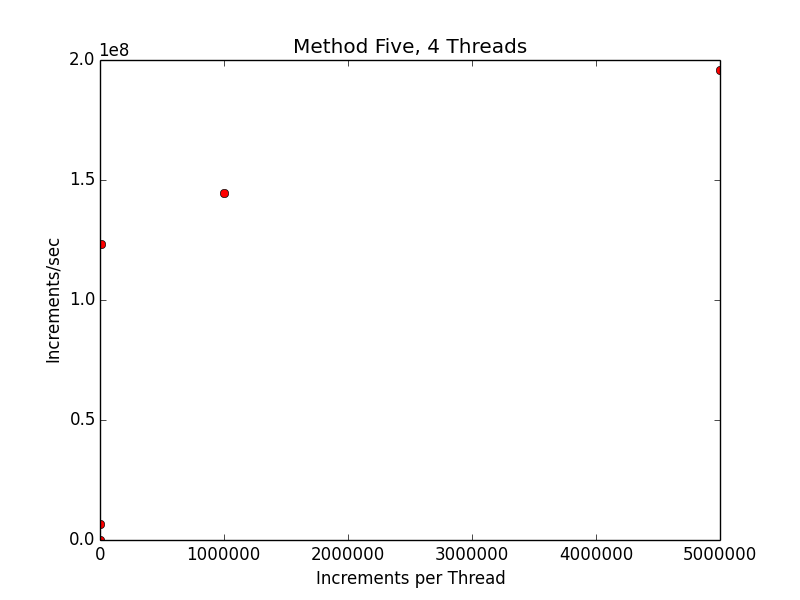
\includegraphics[scale=.5]{Graphs/MethodFive_4Thread.png}

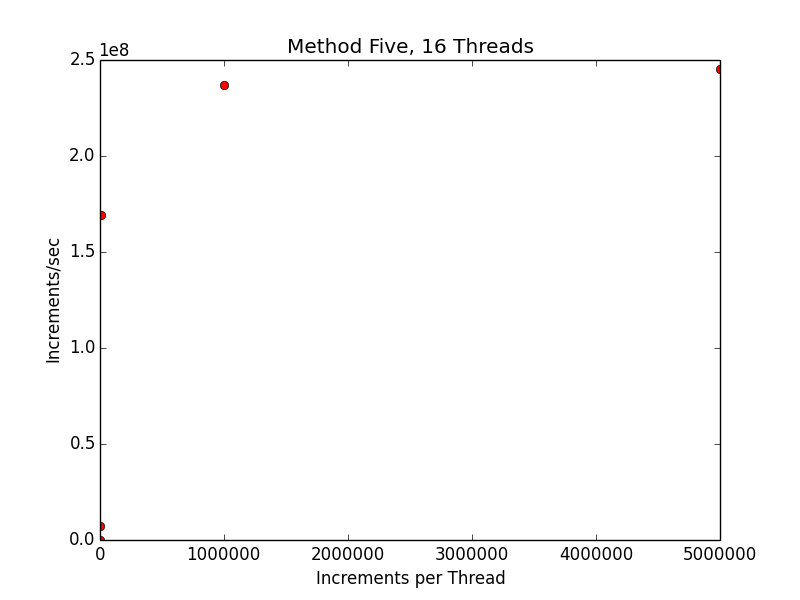
\includegraphics[scale=.5]{Graphs/MethodFive_16Thread.png}

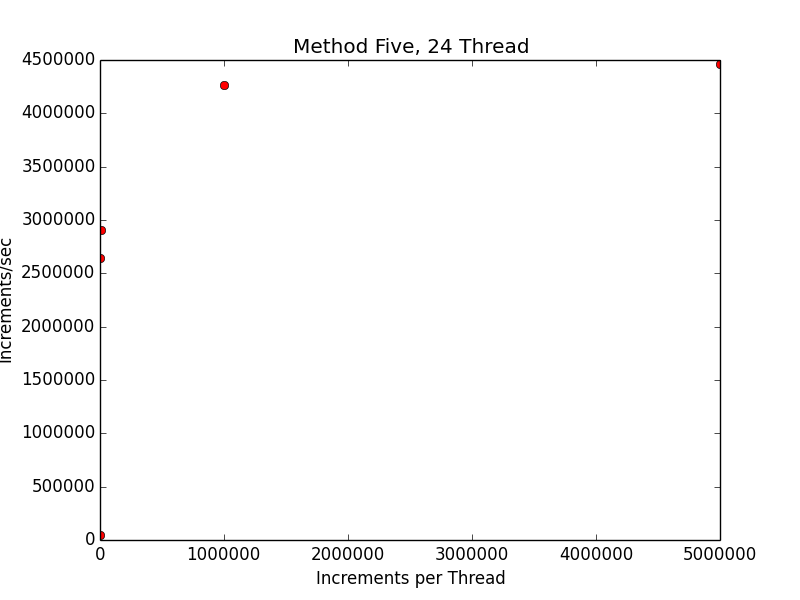
\includegraphics[scale=.5]{Graphs/MethodFive_24Thread.png}

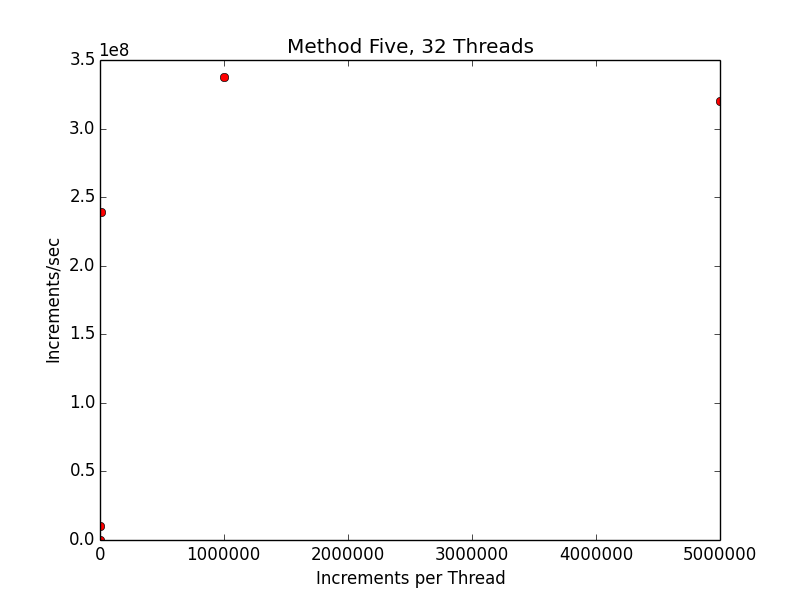
\includegraphics[scale=.5]{Graphs/MethodFive_32Thread.png}

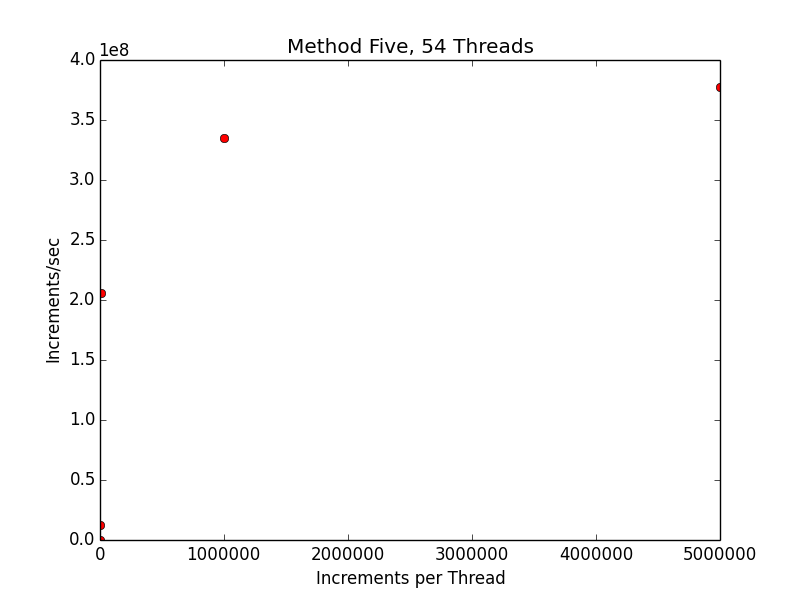
\includegraphics[scale=.5]{Graphs/MethodFive_54Thread.png}


\section{Conclusions}\label{conclusions}
Overall it is apparent from these tests that a form of syncronization is necissary
in order to maintain correctness. While using a mutex did produce correct results
they took much longer. Using an atomic integer completed in a reasonable ammount of
time, and was correct, however the most effective method was by using local variables
in each thread, and then collecting the results. This was effective beacuse it did not
require syncronization methods

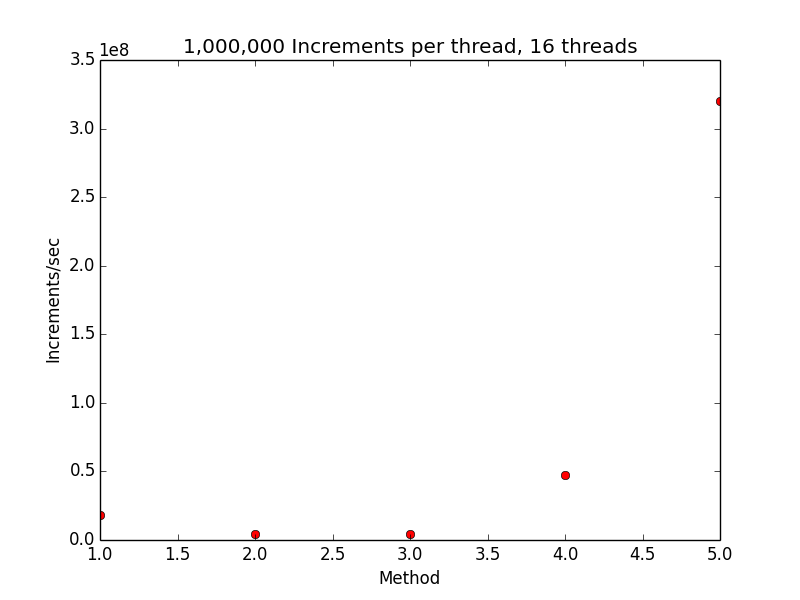
\includegraphics[scale=.5]{Graphs/MethodCmp.png}
\end{document}
